\documentclass[a4paper,twoside,10pt]{article}

\usepackage[francais]{babel}
\usepackage[T1]{fontenc}
\usepackage[utf8]{inputenc}

\usepackage{graphicx} 
\usepackage{qtree} %arbres
\renewcommand{\H}{\mathcal{H}}
\newcommand{\I}{\mathcal{I}}
\newcommand{\B}{\mathcal{B}}
\newcommand{\D}{\mathcal{D}}
\usepackage{amssymb}
\usepackage{amsmath}
\usepackage{amsfonts}
%\usepackage{amsthm}

\usepackage{setspace} %\onehalfspacing       %% 1,5-spacing
%\usepackage{a4wide} %%Smaller margins = more text per page.

%\usepackage{minted}
%% En-têtes précédentes
%\newminted{python}{
%    linenos=true,
%    bgcolor=lightgray,
%    tabsize=4,
%    gobble=8,
%    fontfamily=courier,
%    fontsize=\small,
%    xleftmargin=5pt,
%    xrightmargin=5pt
%}
%
%\usemintedstyle{colorful}
\newenvironment{Q}[1]{%
\vspace{1ex}
\underline{\textbf{Question #1\\}}
\newline
}{
\vspace{2ex}
}

\title{Entropie et codage de source}
\author{Alice Andrès, Quentin Soubeyran}

\begin{onehalfspacing}
\begin{document}
\maketitle

\section{Entropie d'une distribution de probabilité}

\subsection{Cadre de travail et idée intuitive}
\begin{Q}{1}
Comme $X \sim \B(N,p)$, on a :
\[
p(x) = {N \choose k} p^k (1-p)^{(N-k)}
\]
%\begin{align*}
%\H(x) &= - \sum_{k=0}^N p(x) \log_2(p(x)) \\
%	&= - \sum_{k=0}^N {N \choose k} p^k (1-p)^{(N-k)} \log_2 \left({N \choose k} p^k (1-p)^{(N-k)}\right) \\
%	&= \log_2(N!) \sum_{k=0}^N {N \choose k} p^k (1-p)^{(N-k)} \left( \log_2\left(k!(N-k)!\right) \right) \\
%	&\qquad- \log_2(p) \sum_{k=0}^N {N \choose k} p^k (1-p)^{(N-k)} k \\
%	&\qquad- \log_2(1-p) \sum_{k=0}^N {N \choose k} p^k (1-p)^{(N-k)} (N-k) \\
%	&= \log_2(N!) \sum_{k=0}^N {N \choose k} p^k (1-p)^{(N-k)} \left( \log_2\left(k!(N-k)!\right) \right) \\
%	&\qquad-pN\log_2(p) - (1-p)N\log_2(1-p) 
%\end{align*}

On peut ainsi calculer l'entropie $\H$ de $X$ numériquement. Simulons $n$ variables aléatoires et calculons la différence entre $2^{-n\H}$ et $p_X(x_1)...p_X(x_n)$.

\begin{center}
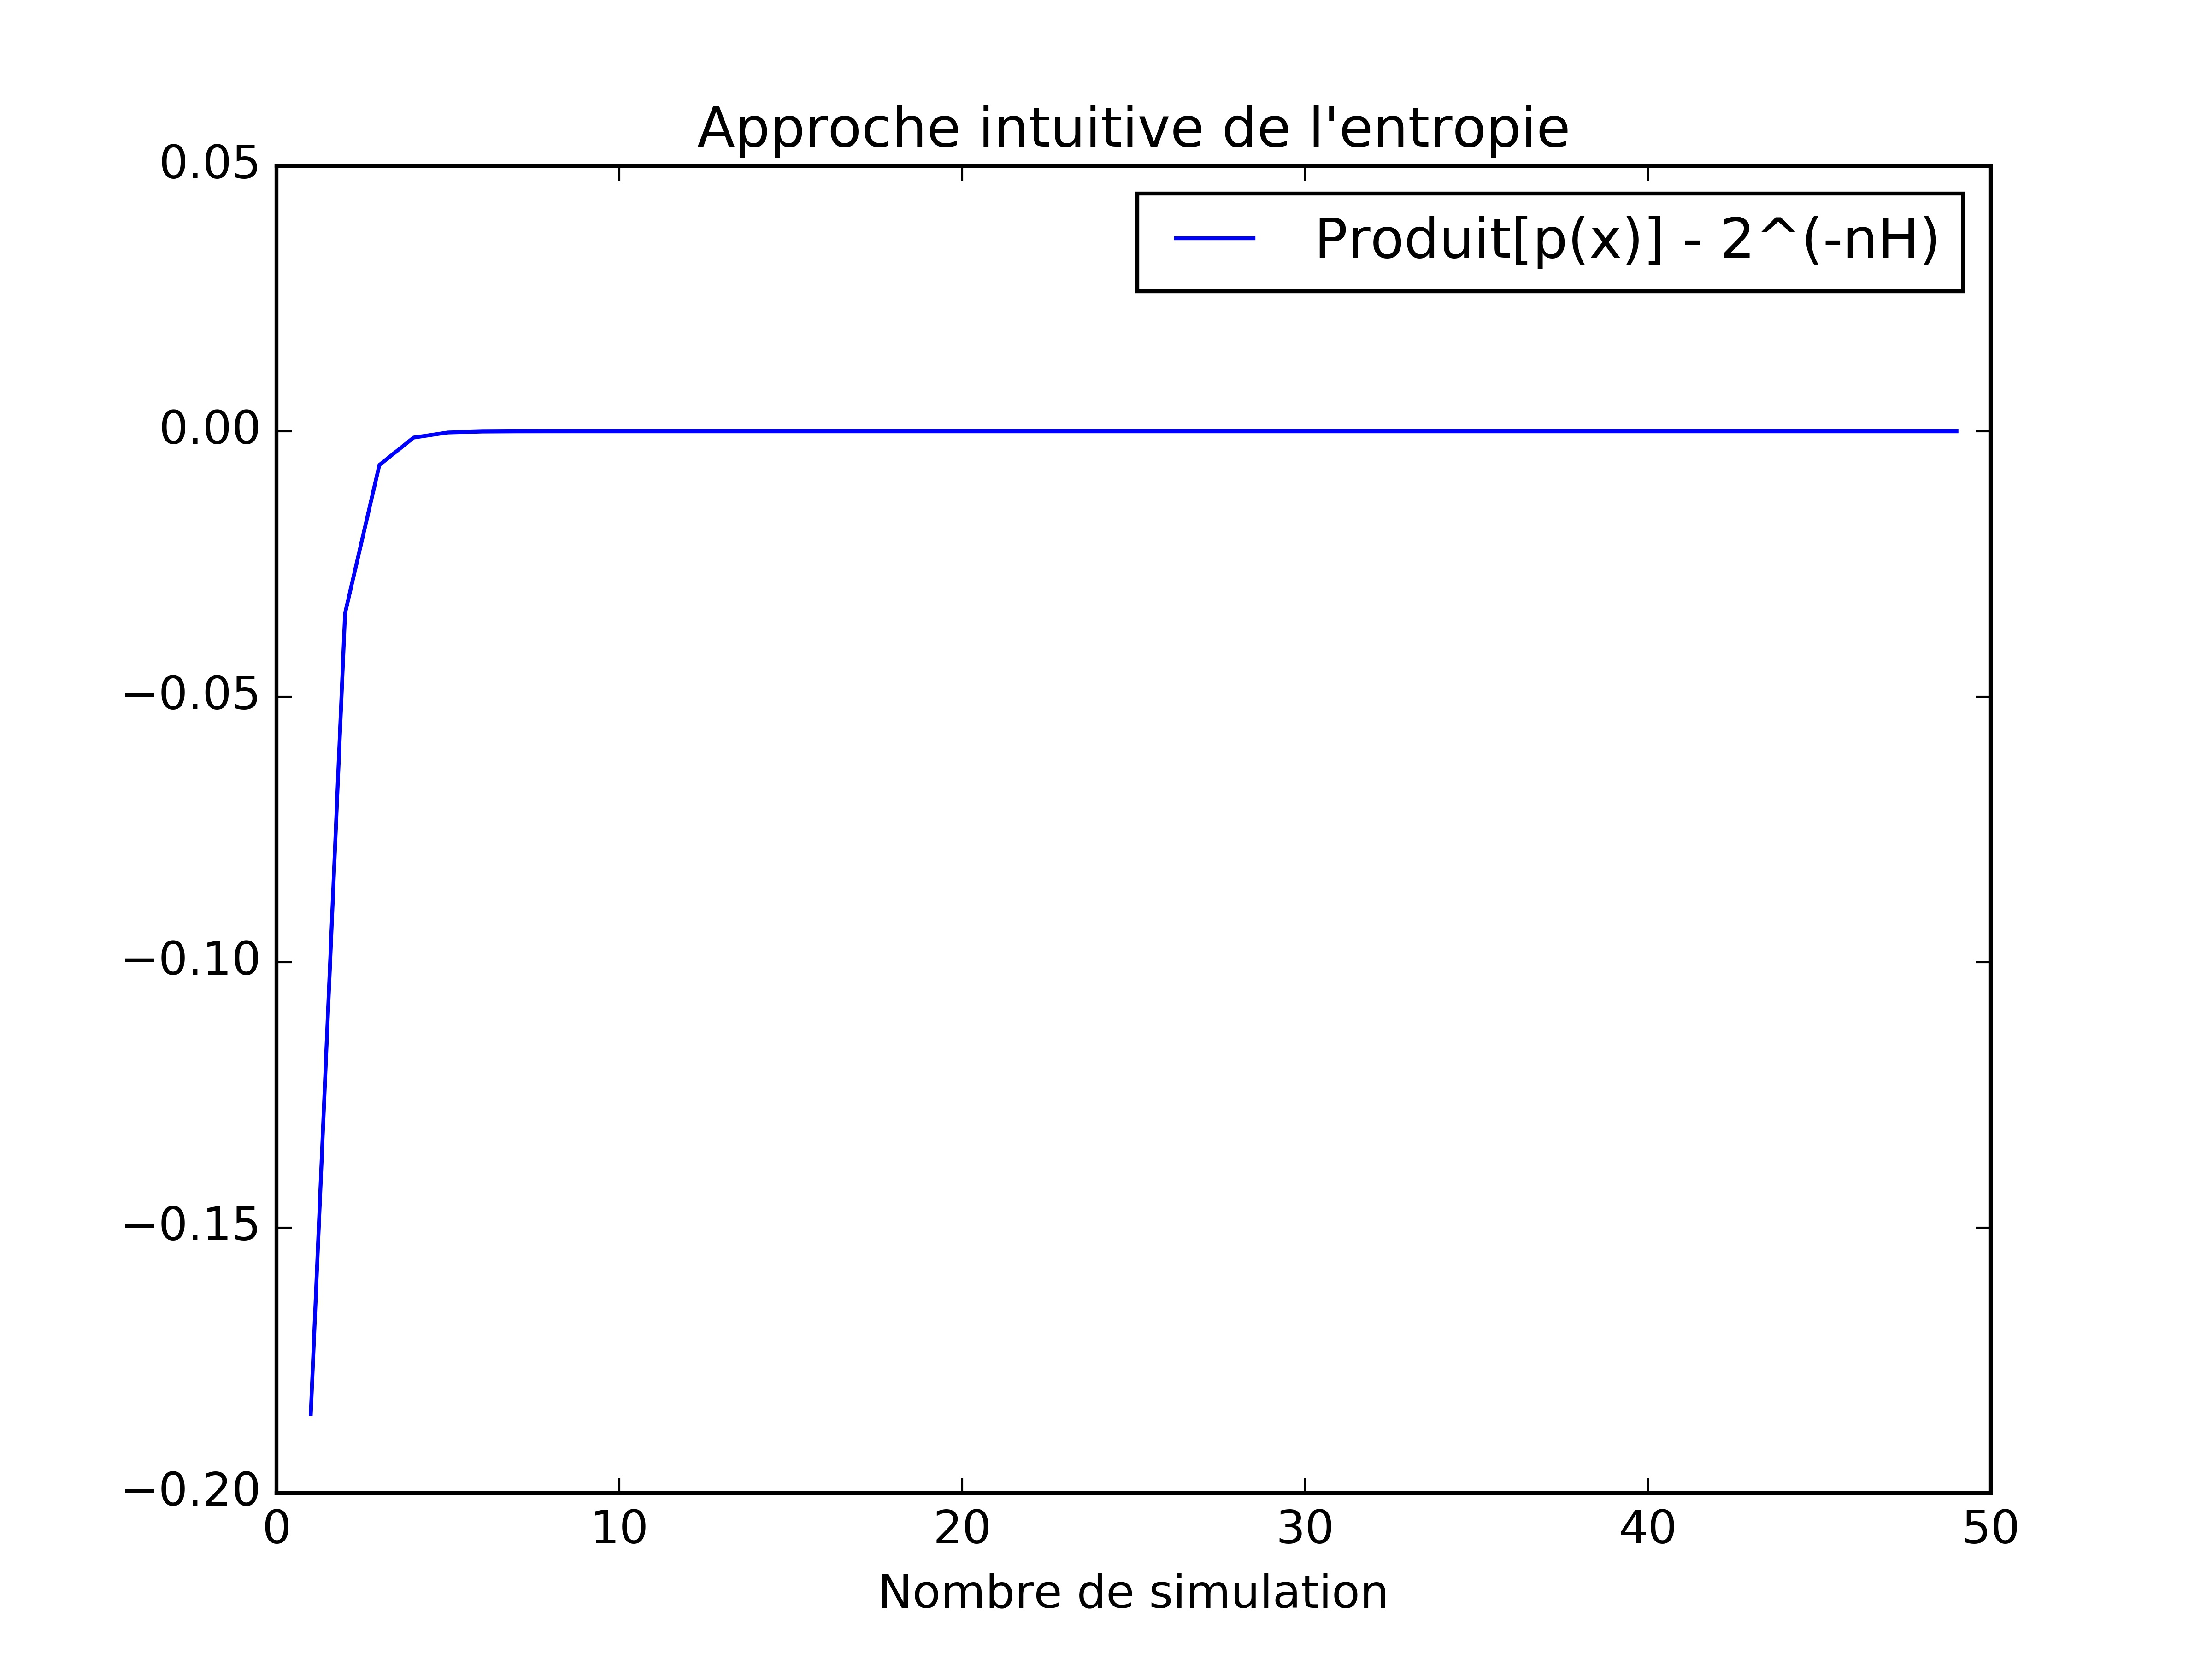
\includegraphics[width=\textwidth]{Q1.jpg}
\end{center}

On remarque que la différence converge rapidement vers 0 (cette observation est confirmée pour un grand nombre de simulation, 10000 par exemple).


\end{Q}
\subsection{Entropie relative et information mutuelle}
\begin{Q}{2}
\[
\D(\B(a)||\B(b))
= a \operatorname{log_2}(\frac{a}{b}) + (1-a) \operatorname{log_2}(\frac{1-a}{1-b})
\]

D'où
\[\D(\B(a)||\B(b))  - \D(\B(b)||\B(a)) 
= (a+b)\log_2{\frac{a}{b}} + (2-a-b)\log_2{\frac{1-a}{1-b}}
\]

Or pour $a = \frac{1}{4}$ et $b = \frac{1}{2}$, 
\[
\D(\B(a)||\B(b))  - \D(\B(b)||\B(a))
= \frac{3}{4} \log_2{(2)} + \frac{5}{4} \log_2{(\frac{3}{2})} \neq 0
\]


Ainsi, dans le cas général, $ \D (p||q) \neq \D(q||p)$
\end{Q}

\begin{Q}{3a}
La fonction $- \log_2$ est strictement convexe. Alors, d'après l'inégalité de Jensen,
\begin{align*}
\sum_{x \in E} \operatorname{p}(x) \left(
	- \operatorname{log_2}\frac{q(x)}{p(x)}
	\right) &\geq 
		-\log_2{\sum_{x \in E} p(x) \frac{q(x)}{p(x)}} \\
&\geq -\operatorname{log_2} \sum_{x \in E}q(x) \\
&\geq 0 \\
\end{align*}
Ainsi $D(p||q) \geq 0$.
La stricte convexité de $-\log_2$ permet de conclure qu'il y a égalité si et seulement si $\forall x \in E$, $p(x) = q(x)$, soit $p=q$. 
\end{Q}

\begin{Q}{3b}

D'après Q3a, $\I(X,Y) = \D(p_{(X,Y)} || p_X \otimes p_Y) \geq 0$

Avec égalité si et seulement si $p_{(X,Y)} = p_X \otimes p_Y$ soit $X$ et $Y$ indépendantes.
\end{Q}

\begin{Q}{4a}
\begin{align*}
\\H(X,Y) &= - \sum_{x,y \in E^2}  p_{X,Y}(x,y)\log_2{(p_{X,Y}(x,y))} \\
	&= -\sum_{x \in E} \sum_{y \in E} p_X(x) p_{Y|X = x}(y) \log_2{p_X(x)}
		+ \log_2{p_{Y|X= x}(y)} \\
	&= \H(X) + \sum_{x \in E} p_X(x)
		\left(
			-\sum_{Y \in E} p_{Y|X = x}(y) \log_2{p_{Y|X = x}(y)}
		\right) \\
 = \H(X) + \H(Y|X)
\end{align*}
Et l'on a montré l'égalité.
\end{Q} 
 
\begin{Q}{4b}

\begin{align*}
 \I(X,Y) &= \sum_{(X,Y) \in E²} p_{X,Y}(x,y)
				\log_2{\frac{p_{X,Y}{(x,y)}}{p_X(x)p_Y(y)}} \\
	&= \sum_{(X,Y) \in E²}
		\operatorname{p_X}(x) p_{Y|X=x}(y) \log_2{(p_{Y|X=x}(y))} 
 		- \sum_{(X,Y) \in E²}
 			p_Y(y) p_{X|Y=y}(x) \log_2{(p_{Y}(y))} \\
	&= \H(Y) - \H(Y|X) \\
	&= \H(X) - \H(X|Y) \text{\quad par symétrie des rôles de X et Y)} \\
	&= \H(Y) - \left(\H(X,Y) - \H(X)\right) \text{\quad cf. (Q4a)} \\
	&= \H(X) + \H(Y) - \H(X,Y)
\end{align*}
\end{Q}

\begin{Q}{4c}

D'après Q4b, $\H(X,Y) = \H(X) - \I(X;Y)$ Or $\I(X;Y) \geq 0$

Ainsi, $\H(X,Y) \leq \H(X)$
\end{Q}

\begin{Q}{5a}

On utilise l'algorithme d'inversion de la fonction de répartition pour une loi discrète.

On utilise python pour déterminer un nombre $a$ aléatoirement suivant la loi uniforme, entre 0 et 1, et on pose Y tel que : 
\[
Y = x_i  \iff \sum_{j = 1}^{i-1} p_j < a \leq \sum_{j = 1}^{i} p_{j+1}
\]

On peut appliquer ce principe pour $X \leadsto \B(\frac{1}{3})$

Soit $a \sim \mathcal{U}([0;1])$. Notons aussi $x_0 = 1$ et $x_1 = 0$

Alors $\mathbb{P}(X = x_0) = \frac{2}{3} = \mathbb{P}(a < \frac{2}{3})$ et 
$\mathbb{P}(X = x_1) = \frac{1}{3} = \mathbb{P}(a > \frac{2}{3})$.
\end{Q}

\begin{Q}{5b}
Voir le code dans le fichier Q5.py.
\end{Q}

\begin{Q}{6a}
Voir le code dans le fichier Q6.py.

On obtient \[H(X) \approx 0.6685644431995964 \text{ et } \H(X|Y) = 1,25\]
\end{Q}

\begin{Q}{6b}
Voir le code dans le fichier Q6.py.

On observe, encore un fois, un convergence de $\frac{1}{k} \sum_{i = 1}^{k} \H(X|Y = y_i)$ vers $\H(X|Y) = 1,25$.

\begin{center}
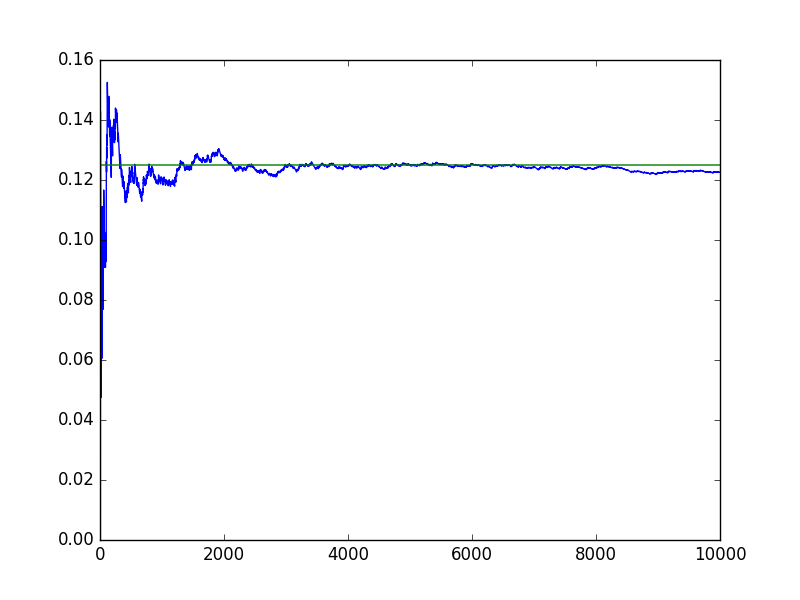
\includegraphics[width=\textwidth]{Q6b.png}
\end{center}

\end{Q}

\begin{Q}{6c}
On obtient \[\H(X|Y = 0) = 0 \text{ et } \H(X|Y = 1) = 1 > \H(X) \approx 0.6685644432 \]
\end{Q}

\section{Application au codage de source}
\subsection{Théorème du codage de source}

\begin{Q}{7a}

\begin{align*}
\D(p_X||q) &= \sum_{x \in E}p_X(x)log_2(\frac{p_X(x)}{\frac{1}{c}d^{-l(x)}}) \\
&\geq 0
\end{align*}

Alors
\begin{align*}
\sum_{x \in E}p_X(x)log_2(p_X(x)) &\geq  -\sum_{x \in E}p_X(x)l(x)log_2(d) + \sum_{x \in E}p_X(x)log_2(\frac{1}{c}) \\
 &\iff\\
-\H(X) &\geq -log_2(d) \mathbb{E}(X) + log_2(\frac{1}{c})
\\ &\geq -log_2(d) \mathbb{E}(X) \texttt{\quad(car} \leq 1 \textsc{)}
\end{align*}

D'où $\frac{\H(x)}{log_2(d)} \leq \mathbb{E}[l(X)]$
 
Le cas d'égalité se déduit de celui de $\D$, et a lieu pour $p_X = q$, soit les $p_X(x)$ sont des puissances négatives de $d$.
\end{Q}

\begin{Q}{7b}
Soit $p$ une loi de probabilité telle que qui s'écrit $p_X(x) = \frac{1}{c}d^{-n_x}$ avec $c = \sum_{x \in E} d^{-n_x}$.

Cas 1 : $c \leq 1$ Prenons $\forall x \in E, l_0(x) = n_x$

Cas 2 : $c > 1$ Alors soit $k$ tel que $\frac{c}{d^k} \leq 1$

$p_X(x) = \frac{d^k}{c}d^{-n_x - k}$, avec $\sum_{x \in E} d^{-n_x - k} \leq \frac{c}{d^k} \leq 1$

Posons alors $\forall x \in E, l_0(x) = n_x + k$

Cette application vérifie l'inégalité de Kraft-McMillan, et vérifie le cas d'égalité de la question Q7a d'après les calculs
précédents pour $q$ définie à partir de la fonction $l_0$.
\end{Q}

\begin{Q}{7c}
La fonction puissance étant bijective sur $\mathbb{R^+}$, on a :
\[
\forall x \in E, \exists \alpha_x, \quad p_X(x) = d ^{\alpha_x}
\]
Posons $c$ et $\beta$ tels que :
\[
c = \sum_{x \in E} d ^{\alpha_x} = d^\beta
\]

Alors
\[
\forall x \in E, \quad p_X(x) = \frac{1}{c} d^{-(\beta - \alpha_x)}
\]
On pose donc
\[
l_0(x) = \beta - \alpha_x
\]
D'où
\begin{align*}
\mathbb{E}[\overline{l_0}(X)] &= \sum_{x \in E} \overline{l_0}(X) \mathbb{P}(X=x)\\
&< \sum_{x \in E} l_0(X)\mathbb{P}(X=x) + \sum_{x \in E}\mathbb{P}(X=x)
\end{align*}
Or d'après la question Q7a, la forme de $p_X(x)= \frac{1}{c} d^{-(\beta - \alpha_x)}$ assure :
\[
\frac{\H(X)}{\log_2(d)} = \mathbb{E}[l(X)] \text{\quad puisque } \D(p_X||p_X) = 0
\]
On en conclut :
\[
\mathbb{E}[\overline{l_0}(X)] < \frac{\H(X)}{\log_2(d)} + 1
\]
\end{Q}

\subsection{Mise en oeuvre de l'algorithme - L'algorithme de Huffman}

\begin{Q}{9a}
Voici le tableau des occurrences.

\begin{center}
\vspace{1ex}
\begin{tabular}{|c|c|c|c|c|c|}
\hline
a & b & c & d & e & f \\
\hline
2 & 3 & 1 & 2 & 2 & 1 \\
\hline
\end{tabular}
\vspace{1ex}
\end{center}

On choisit c et f

\begin{center}
\vspace{1ex}
\begin{tabular}{|c|c|c|c|c|}
\hline
a & b & d & e & cf \\
\hline
2 & 3 & 2 & 2 & 2 \\
\hline
\end{tabular}
\vspace{1ex}
\end{center}

On choisit e et cf

\begin{center}
\vspace{1ex}
\begin{tabular}{|c|c|c|c|}
\hline
a & b & d & ecf \\
\hline
2 & 3 & 2 & 4 \\
\hline
\end{tabular}
\vspace{1ex}
\end{center}

On choisit a et d

\begin{center}
\vspace{1ex}
\begin{tabular}{|c|c|c|}
\hline
b & ad & ecf \\
\hline
3 & 4 & 4 \\
\hline
\end{tabular}
\vspace{1ex}
\end{center}

On choisit b et ad

\begin{center}
\vspace{1ex}
\begin{tabular}{|c|c|c|}
\hline
bad & ecf \\
\hline
7 & 4 \\
\hline
\end{tabular}
\vspace{1ex}
\end{center}

On n'a plus que deux éléments, et construisons donc l'arbre en remontant les étapes précédentes.

\Tree [. bad ecf ]

On décompose bad en b et ad

\Tree [. [.bad b ad ] ecf ]

On décompose ad en a et d

\Tree [. [.bad b [.ad a d ] ] ecf ]

On décompose ecf en e et cf

\Tree [. [.bad b [.ad a d ] ] [.ecf e cf ] ]

On décompose cf en c et f

\Tree [. [.bad b [.ad a d ] ] [.ecf e [.cf c f ] ] ]

On en déduit le codage de Huffman : 

\begin{tabular}{|c|c|c|c|c|c|}
\hline
a & b & c & d & e & f \\
\hline
010 & 00 & 110 & 011 & 10 & 111 \\
\hline
\end{tabular}
\end{Q}

\begin{Q}{9b}
Voir le fichier Python Q9.py
\end{Q}

\begin{Q}{9c}
%A toi !
\end{Q}

\begin{Q}{9d}
Le code est disponible dans le fichier Q9.py.
On constate que le langage de Huffman correspond bien à un langage décrit par le Théorème de Schannon, puisqu'il vérifie
la double inégalité (iii)

En effet, on obtient pourun proba uniforme : 
\[ 3.4585110748 \leq 3.54475447545 < 4.4585110748 \]
Et pour la répartition des lettres de la langue française : 
\[ 2.77115542449 \leq 2.83174404962 < 3.77115542449 \]
\end{Q}

\begin{Q}{9e}

Les moyennes obtenues sont de l'ordre de 3, soit très intéressantes par rapport à 8 bit ; surtout lorsque la 
répartition des caractères n'est pas uniforme.

Mais l'alphabet considéré est restreint par rapport à ce que les 8 bits peuvent coder. Il est donc plus pertinent de comparer au nombre
minimal de bits pour coder 11 caractères, qui est de $log_2(11) \approx 3,45$.

On a donc besoin de 4 bits au minimum pour coder ces 11 caractères ; cela est aussi nécessaire avec le codage de Huffman lorsque la 
répartition est uniforme. On gagne cependant un bit lorsques les fréquences sont disparates : 
on passe à 3 bits. ($\lceil \mathbb{E}(l(X)) \rceil $).

\end{Q}

\end{onehalfspacing}
\end{document}
